% --------------------------------------------------------------------

\section{Introduction}

In the past fifteen years, 
there have been rapid advances in the algorithms for combinatorial problems. 
This has been greatly sparked by the development in algebraic techniques for solving the 
multilinear monomial detection problem, that is, 
deciding whether a multivariate polynomial contains a multilinear monomial.
Multilinear monomial detection for parameterized combinatorial problems was 
first introduced by \citeauthor{Koutis05} in an early work 
\cite{Koutis05}, where a set packing problem is 
reduced to multilinear monomial detection.

Namely, the technique of algebraic fingeprinting, soon after  
introduced by \citeauthor{Koutis08} \cite{Koutis08} and further developed by 
\citeauthor{Williams09} \cite{Williams09}, 
has found great success for many combinatorial problems. 
For example with algebraic fingerprints, the $k$-path problem 
that previously could be solved in \bigOstar{4^{k}} time by \citeauthor{Chen07} \cite{Chen07}, 
could be solved in \bigOstar{2^{3k/2}} time \cite{Koutis08}. 
\amnote{What is the meaning of \bigOstar{}?}
This result was quickly improved by \cite{Williams09} \cite{Williams09}, 
who gave an \bigOstar{2^k} algorithm.

\amnote*[inline,nomargin]{This technique was further developed by
\citeauthor{Björklund14} \cite{Björklund14}, who showed ...}{
Of course, this technique was further developed, and soon after in
\cite{Björklund14} Björklund et al. showed an algorithm 
}
\amnote{Note use of \texttt{\textbackslash citeauthor}}
that solved the Hamiltonian problem (Hamiltonicity), i.e., finding whether a given graph contains a simple path that visits 
every vertex, in \bigOstar{1.657^n} time. Soon enough, for $k$-path, an \bigOstar{1.66^k} algorithm was found \cite{Björklund17}. 
\amnote{Did Björklund really develop the technique further? or did he only show
how to apply it to another problem?}
The fastest algorithms for Hamiltonicity before this ran in
\amnote*{$n$ or $k$?}{ \bigOstar{2^n} }
and were known since 1962 \cite{HelKar62}, \cite{Bellman62}.
This was a significant improvement on a problem that had seen no progress in nearly fifty years.

\subsection{Research goals and thesis structure}
\amnote[inline,nomargin]{This section can be shortened to one paragraph}

The goals of this thesis are to find out how multilinear monomial detection is relevant in 
combinatorial problems, and how algebraic fingerprints can be utilized to design faster 
algorithms for problems that use multilinear monomial detection. Also, interesting ideas 
regarding algebraic fingerprints are explored for.

Multilinear monomial detection 
is a fundamental problem, since many important combinatorial problems can be reduced into it 
via a problem specific algebraization. Thus, faster algorithms and new ideas for multilinear monomial detection 
are important.

Multilinear monomial detection is essentially searching for solutions among non-solutions, 
both of which are encoded as monomials in a polynomial. 
The technique of algebraic fingerprinting is present in multilinear monomial detection. 
With algebraic fingerprints, unwanted cancelation of solution monomials due to the characteristic of a field can be prevented. 
Moreover, algebraic fingerprints can be used to cancel non-solution monomials by abusing the characteristic.

In the next subsections, the thesis discusses algebraization and reduction into multilinear monomial detection. 
The section 2 covers preliminaries. In section 3, the thesis discusses general multilinear monomial detection. 
In section 4, some problem specific instances of multilinear monomial detection are given, and clever 
utilizations of algebraic fingerprints are shown. Section 5 concludes the
thesis.

\subsection{Algebrization of combinatorial problems}

A combinatorial problem asks whether a given finite set of objects satisfies some given constraints. 
For example, the $k$-path problem asks for, given a finite set of vertices and edges, 
a simple path of $k$ vertices. The solutions and non-solutions (solution space) to combinatorial problems can be thought of as 
combinations of the given objects.
\amnote*{Probably one can drop the vertices and think only about edges?}{%
The solution space for the $k$-path problem
consists of combinations of $k$ vertices and $k-1$ edges. 
}
A non-solution combination would contain duplicate vertices, or edges that
contain vertices outside the combination.

\amnote[inline,nomargin]{This sounds like a very simple problem... But I guess
the catch is that we want an algorithm with complexity depending only on $k$?}

Algebraization is reducing a given problem into an algebraic form,
\amnote*[inline,nomargin]{that is}{i.e.}, a
question regarding some algebraic property of some algebraic entity. 
In an algebraization of a combinatorial problem, the algebraic entity can be constructed from algebraic elements defined from the 
set of objects given as an input. The motivation behind the construction is some algebraic property that, 
when satisfied, gives a solution to the problem.

\amnote{Somewhere we need to reference the reader to Sect.~2 for non-familiar
terms like multivariate, algebras, etc.}
In \cite{Valiant92}, it was observed that multivariate polynomials in certain algebras have natural combinatorial interpretations. 
Utilizing this idea, \cite{Koutis05} managed to reduce a combinatorial problem
into an algebraic form, that is, multilinear monomial detection. 
First, we introduce multiple variables that 
correspond to elements from the set of objects given as input. 
Then, we construct an arithmetic circuit representing a multivariate polynomial, such that it 
encodes all solutions and non-solutions as multivariate monomials, 
with multilinear monomials corresponding to solutions. 
Thus, the task of finding a satisfying combination to the combinatorial problem has been reduced to 
finding a multilinear monomial from the multivariate polynomial.
It follows that a decision problem is answered by 
the existence of a multilinear monomial, and a counting problem by the number of multilinear monomials.

Appropriate definitions for the variables are problem-specific. In the following section, this thesis gives a 
reduction into multilinear monomial detection, shown in \cite{KouWil15}, 
for the $k$-3D matching problem. Another simple example can be found, for the set packing problem, in \cite{Koutis05}.

\amnote[inline,nomargin]{I would merge the two sections and use the $k$-3D
matching as an example to the explanation above}

\subsection{Reducing $k$-3D matching to multilinear monomial detection}
\label{sect:reduction_example}

The $k$-3D matching problem is defined as follows:

\begin{problem}
  \problemtitle{$k$-\textsc{3D matching}}
  \probleminput{Three disjoint sets $A$, $B$ and $C$, and a set of triples $T\subset A\times B\times C$.}
  \problemquestion{Is there a subset $M\subseteq T$, such that $\abs{M} = k$ and 
  $\forall m \in M$: None of the elements in $m$ appear in
  \amnote*[inline,nomargin]{$M \setminus \{m\}$}{$M\backslash \{m\}$}}
\end{problem}
\amnote{Use \texttt{\textbackslash setminus} instead of \texttt{\textbackslash
backslash}}
\amnote{$T = A \times B \times C$ not allowed?}
\amnote{Either convert $\forall$ into text or what follows into maths}

We begin by defining new variables corresponding to the elements in $A$, $B$ and $C$, 
labeled as $a_i$, $b_j$ and $c_k$, respectively, where $i\in [\abs{A}]$, $j\in
[\abs{B}]$ and $k\in [\abs{C}]$. 
\amnote{Def. of $\abs{\cdot}$?}

For every triple $t \in T$, we define a multilinear monomial $x$ that is a
product of the elements in $t$. 
\amnote{Over what object are we doing multiplication?}
We introduce a set $X$ that satisfies the following:
%\begin{center}$\forall x \in X$: $x = abc$ : $(a, b, c) \in T$.\end{center}
\[
\forall x \in X: x = abc : (a, b, c) \in T.
\]
\amnote{Use \textbackslash[ ... \textbackslash] for display math}
\amnote[inline,nomargin]{Probably meant $\forall x \in X, x = abc ...$?}

Next, we define multivariate polynomials $P_1$ and $P_k$ as follows:
\begin{center}$P_1 = \displaystyle \sum_{X}$ ,   $P_k = P_1^k$.\end{center}
\amnote{Meaning of $\sum_X$?}

Following this construction, we observe that $P_k$, when expanded into a sum of multivariate monomials, 
contains a multilinear term if and only if the original $k$-3D matching instance can be answered in the positive. 
Furthermore, every multilinear monomial in the expanded $P_k$ corresponds to a solution to the problem, and 
the solutions can be directly found from the variables in the multilinear monomial. Thus, 
a successful reduction into multilinear monomial detection has been given for the $k$-3D mapping.

An example instance of $k$-3D matching with this exact algebraization can be found in \cite{KouWil15}. 
TODO: show the example here


\subsection{Problem definition}

The general, parameterized multilinear monomial detection problem is defined as follows: 

\begin{problem}
  \problemtitle{$k$-\textsc{multilinear monomial detection}}
  \probleminput{A commutative arithmetic circuit $A$ over a set of variables $X$ representing a polynomial $P(X)$.}
  \problemquestion{Does the polynomial $P(X)$ extended as a sum of monomials 
  contain a multilinear monomial of degree $k$?}
\end{problem}

Clearly, an upper bound for solving the problem is given by a 
naive expansion of $A$ into $P(X)$ and evaluation of $P(X)$. 
However, this is not optimal: an $N$-degree polynomial will have $2^{\Theta(N)}$ 
possible monomials, and most problems that can use this algebraization, 
have been solved with faster algorithms. %(TODO: quick example?) 
This motivates the detection of multilinear monomials 
without fully expanding $A$ into a sum of monomials.

Since only multilinear terms are important in $P(X)$, 
any squared variable can be instantly discarded as soons as it is formed in $A$. 
This can be achieved with dynamic programming to create a polynomial $P'(X)$ that 
only contains multilinear monomials. Since there are $2^N$ multilinear monomials in $P'(X)$ with 
$N$ variables, this method results in a slightly 
faster algorithm than with naive expansion.

%TODO: Maybe rewrite the algebra here 
%(first quickly in English, then in maths, and maybe label the mapping functions)
However, the underlying problems are usually FPT. This implies that scaling exponentially 
with the number of variables is far from optimal. In order for the complexity of the algorithm to scale 
with the parameter $k$, we can reduce the number of variables by mapping $X$ into $Y$, where 
$\abs{X} \geq \abs{Y}$ and
\amnote*{Def?}{$\abs{Y} \propto k$}, and dynamically evaluate $P(Y)$ instead of
$P(X)$. 
\amnote{$P$ is unchanged, so it still expects $\abs{X}$ arguments...?}

However, since $\abs{X} \geq \abs{Y}$, a multilinear monomial in $P(X)$ may not be multilinear in $P(Y)$. 
For an algorithm to detect a multilinear monomial, it is necessary to use different mappings 
from $X$ into $Y$ until a multilinear monomial survives the mapping. However, the probability 
that any given multilinear monomial survives this mapping is around $e^{-\abs{Y}}$ \cite{KouWil15}. 
This implies that 
\bigOmega{e^{\abs{Y}}} random mappings must be tried for a 
multilinear monomial to survive with a reasonable constant probability. Thus, a 
$k$-multilinear monomial is detected with a 
randomized algorithm in \bigOstar{(2e)^{\abs{Y}}} time, where $\abs{Y} \propto k$.

This is essentially the idea behind color coding introduced by \citeauthor{Alon95} \cite{Alon95}. 
Although here given in this algebraic form for the $k$-multilinear monomial detection, 
color coding is combinatorial, and does not rely on algebraic techniques. 
However, since $k$-multilinear monomial detection is a purely algebraic problem, it is reasonable to 
conjecture that there is an algebraic method for solving it.

Indeed, a faster algebraic method exists; the technique of algebraic fingerprinting 
first introduced by \citeauthor{Koutis08} \cite{Koutis08} and 
further developed by \citeauthor{Williams09} \cite{Williams09} 
solves $k$-multilinear monomial detection in \bigOstar{2^k} time. 
Since the technique focuses on the abstract $k$-multilinear monomial detection, 
to which many parameterized problems can be reduced to, 
it gives a general framework for 
solving parameterized problems \cite{KouWil15}.

\section{Related problems} %TODO: maybe change headline?
\label{sect:related_problems}

The importance of multilinear monomial detection lies in the fact 
that many combinatorial problems, as we see in this section, 
can be reduced to instances of it. 
Thus, solving the general $k$-multilinear monomial detection problem 
efficiently has been of great interest. 
Moreover, the technique of algebraic fingerprints underlie the fastest algorithms 
for all the problems mentioned here. 
Note that only time complexity is discussed here. 
%However, though omitted, space complexities have also been improved with algebraic fingerprinting.

Ideas behind representing combinatorial problems with multivariate polynomials have 
been considered before, e.g., by \citeauthor{Valiant92} \cite{Valiant92} and 
\citeauthor{Koutis05} \cite{Koutis05}. However, 
\citeauthor{Koutis08} was the first one to introduce and apply multilinear monomial 
detection for combinatorial problems, namely the $k$-path and $m$-set $k$-packing problems 
\cite{Koutis08}. For $k$-path, this improved the runtime from 
\bigOstar{4^k} \cite{Chen07} to \bigOstar{2^{3k/2}}, and for $m$-set $k$-packing, 
the runtime was improved from \bigOstar{5.44^{mk}} \cite{Koutis05} to \bigOstar{2^{mk}}.

Soon after, \citeauthor{Williams09} developed this algebraic technique 
for an \bigOstar{2^k} $k$-path \cite{Williams09}, 
from which \citeauthor{KouWil09} \cite{KouWil09, KouWil15} 
gathered and proposed a general 
\bigOstar{2^k} algebraic framework, 
\emph{algebraic fingerprinting}, for $k$-multilinear monomial detection 
as a general technique for 
parameterized combinatorial problems. In their work \cite{KouWil09}, 
\citeauthor{KouWil09} gave faster \bigOstar{2^k} algorithms using this technique for the 
$k$-tree, $k$-leaf spanning tree, and $t$-dominating set problems. %, and an 
%\bigOstar{2^{(m-1)k}} algorithm for the $m$-dimensional $k$-matching problem. 
The runtimes of the previously fastest algorithms for these problems, respectively, were   
\bigOstar{(2e)^k} \cite{Alon95}, \bigOstar{4^k} \cite{Kneis11}, \bigOstar{(4+\varepsilon)^t} \cite{Kneis07}. 

Due to the development in algebraic fingerprinting, 
\citeauthor{Björklund14} \cite{Björklund14} found an \bigOstar{1.657^n} algorithm for 
Hamiltonicity, improving the runtime from \bigOstar{2^n} \cite{Bellman62, HelKar62}, 
by clever algebrization and utilizations of algebraic fingerprints. Using similar 
ideas, \citeauthor{Björklund17} \cite{Björklund17} gave faster algorithms for 
$k$-path, $m$-set $k$-packing, and its special case of 3-set $k$-packing. 
The runtimes for these were \bigOstar{1.657^k}, \bigOstar{2^{(m-2)k}} and \bigOstar{1.493^{3k}}, respectively.

$k$-multilinear monomial detection itself was widely studied by 
\citeauthor{Chen07} \cite{Chen07, Chen11a}, \citeauthor{Chen13a} \cite{Chen13a, Chen11b} 
and \citeauthor{Chen13b} \cite{Chen13b}. TODO: what did they research (deterministic stuff, primality of the field) 
(In this thesis though, we focus on the randomized technique of algebraic fingerprinting.)

TODO: deterministic multilinear detection

TODO: constrained multilinear detection (weights? functional motifs for biological networks)

TODO: parallelization (MIDAS?)

Stuff: Fast graph scan statistics, temporal graphs, 

\section{Preliminaries}
\label{sect:prelims}

It is necessary to recall basic algebraic concepts and common notation 
before further discussing multilinear monomial detection and algebraic fingerprinting. 
Section \ref{sect:prelims_algebra} gives definitions for some necessary algebras 
and algebraic concepts. Section \ref{sect:prelims_circuits} outlines arithmetic circuits. 
Section \ref{sect:prelims_other} gives a table of other notation and terminology used 
throughout the thesis.

\subsection{Algebra} 
\label{sect:prelims_algebra}

\textbf{Groups.} A \emph{group} $\mathbf G$
is a tuple $(G, +)$, where $G$ is a set of elements, 
$+ \colon G \times G \to G$ 
is a binary operation closed under 
the elements in $G$, $+$ is associative, every element $g \in G$ 
has an inverse $g^{-1}\in G$, and $G$ contains 
an identity element $e$ such that $g + e = g$, $g + g^{-1} = e$ and $e = e^{-1}$. 
Moreover, $\mathbf G$ is called \emph{Abelian} if 
$+$ is also commutative. A group is called \emph{multiplicative} if the operation 
is written as multiplication.

\textbf{Rings.} A \emph{ring} $\mathbf R$ is a triple $(R,+,\cdot)$, 
where $(R, +)$ is an Abelian group, and $\cdot \colon R \times R \to R$ 
is a binary operation closed under $R$. We call the binary operations $+$ and $\cdot$ 
addition and multiplication, respectively. A \emph{commutative ring} has commutative multiplication. 

Note, from here on we may use a bold typeface to represent either the set of elements 
or the algebraic structure itself, i.e., 
we may use expressions such as $u \in \mathbf{R}$, where $\mathbf{R} = (R,+,\cdot)$ and $u \in R$. 
Moreover, multiplication may be denoted by juxtaposition for brevity: $a\cdot b = ab$. 

$\mathbf{R}$ must contain a multiplicative identity 
$\mathbf{1} \in \mathbf{R}$ such that $\forall a \in \mathbf{R} \colon a \cdot \mathbf{1} = a$. 
We notate the additive identity $e$ 
%required for the group%
as $\mathbf{0}$ from here on. 
Observe that for any $R \neq \{\mathbf{0}\}$, $\mathbf{1} \neq \mathbf{0}$. 
Left and right distributive laws hold for rings, i.e., 
\[
  \forall a, b, c \in \mathbf{R} \colon a \cdot (b + c) = (ab) + (ac) \land (b + c) \cdot a = (ba) + (ca).
\]
$u \in \mathbf{R}$ is called \emph{unit} if it holds 
that $\exists v \in \mathbf{R} \colon uv = vu = \mathbf{1}$, 
i.e., it has a multiplicative inverse $v \in \mathbf{R}$.

\textbf{Fields.} A \emph{field} $\mathbf{F} = (F, +, \cdot)$ is defined with the following conditions:
\begin{itemize}
  \item $(F, +)$ is an Abelian group
  \item $(F\backslash \{\mathbf{0}\}, \cdot )$ is an Abelian group
  \item Left and right distributive laws hold for $\mathbf{F}$.
\end{itemize}

Equivalently, a ring is a field if every non-zero element is unit, $\mathbf{1} \neq \mathbf{0}$, 
and multiplication is commutative. 
The \emph{characteristic} of a field $\mathbf{F}$ is defined as follows:
\begin{equation}
  char(\mathbf{F}) =
    \begin{cases}
      min\{n \in \N \colon n \cdot \mathbf{1} = \mathbf{0} \}\\
      0 & \text{if such $n$ does not exist}\\
    \end{cases}       
\end{equation}

Note, that a field $\mathbf{F}$ with 
characteristic 2 satisfies the following:
\[
  \forall u \in \mathbf{F} \colon u + u = u \cdot (\mathbf 1 + \mathbf 1) = u \cdot \mathbf 0 = \mathbf 0
\]
Throughout the thesis we may use language such as \emph{cancelation due to characteristic} to 
refer to the fact that an element $f \in \mathbf{F}$ may cancel itself out in an expression if 
$\mathbf{F}$ has non-zero characteristic. 
We mainly use characteristic 2 in this thesis, and thus, we may say that 
$f$ cancels out due to characteristic when 
it has an even coefficient: 
$f + f + f + f = 4f = 2f + 2f = \mathbf{0} + \mathbf{0} = \mathbf{0}.$

Characteristics are prevalent in \emph{finite fields}, where the set of elements is finite. 
A simple example of a finite field is $\Z_2 = (\{\mathbf{0}, \mathbf{1}\}, +, \cdot)$, where 
the operations are standard addition modulo 2, and standard multiplication. 

Finite fields can be noted as $GF(p)$, called \emph{Galois fields}, where the field is unique 
up to \emph{isomorphism} if $p$ is a prime or a power of some prime. 
An isomorphism $\kappa \colon \mathbf{A} \to \mathbf{B}$ 
is a bijective mapping that satisfies 
$\forall u,v \in \mathbf{A} \colon \kappa(uv) = \kappa(u)\kappa(v) \wedge \kappa(u+v) = \kappa(u)+\kappa(v).$ 
Thus, if we only care for the relations between the elements, we may say that isomorphic algebras are 
equivalent for us. 
Note that if $p$ is prime and $k \in \N$, the characteristic of $GF(p^k)$ is $p$. 
%Moreover, the non-zero elements of a finite field form a multiplicative group.

\textbf{Polynomial rings and multilinearity.} 
A \emph{polynomial ring} in $X$, noted as $\mathbf{K}[X]$,
is a ring of polynomials with indeterminates (or variables) from $X$ and 
coefficients from the commutative ring $\mathbf{K}$. 
In this thesis, we only handle \emph{multivariate} 
polynomials, i.e., polynomials that have $\abs{X} = n > 1$. 

A \emph{monomial} in $X$ is of the form 
$X_1^{a_1}X_2^{a_2}\cdots X_n^{a_n}$, where $X_i \in X$ and $a_i \in \N$ marks the exponent. 
A monomial is \emph{multilinear} if 
$\forall i \in \{1, \ldots, n\} \colon a_i = 0 \vee a_i = 1$. 
The \emph{degree} of a monomial $m$ 
is the sum of the exponents: $deg(m) = \sum_{i=1}^n a_i$. 
Any element $P$ of such polynomial ring is a finite linear combination of these monomials 
with coefficients $k \in \mathbf{K}$: 
\[
  P = \displaystyle \sum_p k_p(X_1^{a_{1,p}} \cdots X_n^{a_{n,p}})
\] 
Alternatively, a polynomial ring $\mathbf{K}[X]$ can be thought of as a vector space with 
the all the monomials as a basis. 
Polynomial rings have three operations: addition, multiplication 
and scalar multiplication. In terms of vectors, addition and scalar multiplication follow 
the standard addition and scalar multiplication for vectors. 
Note that the scalar value must be in $\mathbf{K}$. 
The multiplication is defined as follows: 
let $M(X)$ denote the set of all monomials in $X$, and 
$P_d$ denote a polynomial in $\mathbf{K}[X]$ of the form $P_d = \sum_{m \in M(X)} d_m m$, 
where $d_m \in \mathbf{K}$. Then, 
\[
  \forall P_a,P_b \in \mathbf{K}[X] \colon P_a \cdot P_b = (\displaystyle \sum_{m \in M(X)} a_m m)
  \cdot (\displaystyle \sum_{n \in M(X)} b_n n) = 
\]

\emph{Evaluation of a polynomial} $P$ at $Z$ is denoted $P(Z)$, where 
$Z \subset \mathbf{R}$ is a set of elements from a ring $\mathbf{R}$ containing $\mathbf{K}$. 
Evaluating at $Z$, i.e., assigning indeterminates $X$ to $Z$, defines an 
element from the ring $\mathbf{R}$, as $P(Z) \in \mathbf{R}$. We may note the unevaluated 
polynomial as $P(X)$ to highlight the set of indeterminates. 
Moreover, in this thesis we mainly use elements of \emph{group algebras} 
for evaluation; $\mathbf{R} = \mathbf{K}[\mathbf{G}]$, where $\mathbf{G}$ is a 
multiplicative group.

\textbf{Group algebras.} A group algebra is very similar to a polynomial ring, and 
is also noted as $\mathbf{R}[\mathbf{G}]$, where $\mathbf{R}$ is a commutative ring and 
$\mathbf{G}$ is a multiplicative group. A group algebra may be thought of as a 
polynomial ring $\mathbf{R}[X]$, where the indeterminates $X$ form a multiplicative group $\mathbf{G}$. 
The elements and operations in a group algebra have the same form as those in a polynomial ring, 
with the exception that instead of summing over monomials in $X$, 
we sum over the elements of $\mathbf{G}$.

Note that $\mathbf{0} \in \mathbf{R}[\mathbf{G}]$ corresponds to a 
polynomial $P \in \mathbf{R}[\mathbf{G}]$ with zero-coefficients, and 
$\mathbf{1} \in \mathbf{R}[\mathbf{G}]$ corresponds to the identity element of $\mathbf{G}$. 

%TODO: Cygan, p. 337

\subsection{Arithmetic circuits}
\label{sect:prelims_circuits}

Computing arithmetic expressions such as polynomial evaluations 
can be represented by \emph{arithmetic circuits}, that is, 
connected acyclic directed graphs, where terminal vertices correspond to initial and output values, 
and other vertices correspond to \emph{arithmetic gates}, i.e., arithmetic operations. 

In this thesis, we only consider \emph{addition} and \emph{multiplication} gates. 
These gates correspond to the binary operations of the underlying algebra  
which the arithmetic expression is evaluated over and given initial values from. Thus, 
the addition and multiplication gates may have \emph{fan-in two} and \emph{fan-out one}, 
i.e., each gate-vertex has three edges connected to it: two as an input, and one as an output. 
If the underlying algebra is commutative, we may call the arithmetic circuit a \emph{commutative circuit}. 
%However, since we are using mainly commutative algebras in this thesis, we may define the 
%gates for binary operations to have unbounded fan-in. 

For example, an abstract evaluation of a polynomial $P$ in $\Z[\{a,b,c,d\}]$ of the form 
$P = (ab+cd)^2$ is given by the arithmetic circuit presented in Figure \ref{fig:circuit_example}. 

\begin{SCfigure}[0.5][h]
  \caption{A circuit for evaluating $(ab+cd)^2$. 
  Note that the input terminals have been copied for clarity.}
  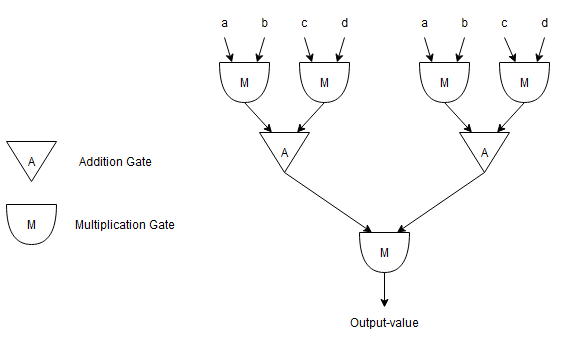
\includegraphics[width=0.7\textwidth, height=5.5cm]{arithmetic_circuit_EXAMPLE.png}
  \centering
  \label{fig:circuit_example}
\end{SCfigure}

\subsection{Notation and other terminology} 
\label{sect:prelims_other}

The following table holds useful notation and their definitions. 
The terms and notation are given on the left, and their definitions on the right.

\begin{tabularx}{\textwidth} { 
  %| 
  X %|
  X %| 
  }
 \hline
 $k$-multilinear monomial & a multilinear monomial that has a degree of $k$ \\
 \hline
 sum of monomials form & an expression for a polynomial $P(X)$ where there are no 
 polynomial multiplications present, i.e., the expression consists of only additions between monomials \\
 \hline
 $\mathcal{O}$* & hides factors polynomial to the input size, e.g., \bigO{n^3k^n} = \bigOstar{k^n} \\
 \hline
 FPT & A class of \emph{fixed parameter tractable} problems, i.e., parameterized problems that 
 can be solved in polynomial time if the parameter is fixed \\
 \hline
 Deterministic algorithm & Given a fixed input, a \emph{deterministic} algorithm always gives the same output \\
 \hline
 Randomized algorithm & A \emph{randomized} algorithm relies on pseudorandom 
 functions, and may not produce the same outputs for a fixed input\\
 \hline
 Schwartz-Zippel lemma & TODO: give here or in the context? \\
 \hline
 term & def \\
 \hline
\end{tabularx}

%\clearpage
\section{General multilinear monomial detection}

The detection of multilinear monomials in a multivariate polynomial is a fundamental problem, 
since many important problems can be reduced to it, 
as seen in Section \ref{sect:related_problems}. 
Therefore, any progress in general multilinear monomial detection implies 
faster algorithms for the problems mentioned in Section \ref{sect:related_problems}.

In this section, 
we discuss the algebraic ideas by \citeauthor{KouWil09} \cite{Koutis08, Williams09, KouWil09} 
for the $k$-multilinear monomial detection. 
In Section \ref{sect:algebraic_fingerprinting}, 
we dive into the technique of algebraic fingerprinting, and 
see the ideas and implementations of \citeauthor{KouWil09}. 
In Section \ref{sect:complexity} we briefly discuss the time and space complexity 
of the general algebraic framework given by algebraic fingerprinting. 
Finally, Section \ref{sect:limits} discusses the limits of algebraic fingerprinting.

As a prelude for the following sections, recall the relevant problem definition: 
\begin{problem}
  \problemtitle{$k$-\textsc{multilinear monomial detection}}
  \probleminput{A commutative arithmetic circuit $A$ over a set of variables $X$ representing a polynomial $P(X)$.}
  \problemquestion{Does the polynomial $P(X)$ extended as a sum of monomials 
  contain a multilinear monomial of degree $k$?}
\end{problem}

\subsection{Algebraic fingerprinting}
\label{sect:algebraic_fingerprinting}

The idea of discarding squared variables as soon as they are formed in $A$ 
can be expressed algebraically: any squared variable should be identical to
zero. 
\amnote{Quotient ring}
\begin{equation}
  \label{eq:squared_to_zero}
\forall x \in X: x^2 = \mathbf{0}
\end{equation}
This implies that any non-multilinear monomial will evaluate to zero in $P(X)$, since 
any non-multilinear monomial $q$, assuming commutativity, can be written as $x^2q'$ 
for some $x \in X$, and \amnote*{$\mathbf{0}q'$?}{$x^2q' = \mathbf{0}q = \mathbf{0}$}. 
Therefore, $P(X)$ will identically evaluate to zero if there are no multilinear monomials, 
i.e., there exist no solutions to the original problem.

This is the basis of algebraic multilinear monomial detection introduced by 
\citeauthor{Koutis08} \cite{Koutis08}, or later referred to as \emph{algebraic fingerprinting} \cite{KouWil15}: 
we evaluate $P(X)$ over some algebra $\mathbf{G}$, and detect a multilinear monomial from 
the value returned by this evaluation. Ideally, with any $\gamma \colon X \to
G$,
\amnote*{What is $X'$?}{
$P(X')$ representing $P(X)$ over $\mathbf{G}$ by $\gamma$
}
and $w \neq \mathbf{0}$, 
\amnote{Evaluation under $\gamma$ needs its own notation, e.g.,
$\varphi_\gamma(P)$}

\begin{equation}
  \label{eq:polynomial_identity}
  P(X') =
    \begin{cases}
      \mathbf{0} & \text{if no multilinear monomials exist}\\
      w & \text{otherwise}\\
    \end{cases}       
\end{equation}

In the following subsections, we specify an appropriate algebra such that 
(\ref{eq:polynomial_identity}) is met, as well as some requirements for efficiency. 
Then, we discuss the works of \citeauthor{Koutis08} and \citeauthor{Williams09} \cite{Koutis08, Williams09}, 
and see how these specifications were implemented.

This thesis refers to the general framework \cite{KouWil09, KouWil15} by these 
authors as algebraic fingerprinting. However, algebraic fingerprinting can also 
be used to refer to the idea behind solving a problem 
with multilinear monomials canceling out due to characteristic, 
which is discussed here in Section \ref{sect:fingerprints}.

\subsubsection{Specifications for the algebra}
\label{sect:algebra_specs}

We have arrived at an important task for multilinear monomial detection: 
find a \amnote*{field or algebra?}{field} $\mathbf{G}$ for 
the assignment $\gamma \colon X \to \mathbf{G}$ to meet 
(\ref{eq:squared_to_zero}) and thus the first equality in (\ref{eq:polynomial_identity}). 
We specify for fields since rings are not enough for multilinear monomial detection; 
$\mathbf{G}$ should have
\amnote*{How about a commutative ring then?}{commutative multiplication} in order for (\ref{eq:squared_to_zero}) 
to be effective. The ordering of indeterminates in monomials is generally unknown, 
since the specific algebrization into multilinear monomial detection 
is abstracted away. %Specifying for commutativity also makes it significantly 
%easier to algebrize problems into arithmetic circuits. 

For the second equality in (\ref{eq:polynomial_identity}), it is necessary that multilinear 
monomials in $P(X)$ can map to multilinear monomials in $P(X')$, i.e., it must
be that 
\amnote{Isn't $P(X')$ the evaluation of $P(X)$ under $\gamma$? If so, then
$P(X')$ is just an element of $\mathbf{G}$, not a polynomial}
$k \leq \abs{G}$, where $k$ is the degree of the monomials. 
Moreover, multilinear monomials 
should not evaluate to $\mathbf{0}$ over $\mathbf{G}$, and more specifically, 
$w$ should not be identical to $\mathbf{0}$.

These are the necessary specifications for the field $\mathbf{G}$ for algebraic multilinear monomial detection. 
However, this algebraic detection must be faster than color coding for it to be useful. 
Therefore, further requirements are necessary: (a) the binary operations of $\mathbf{G}$ 
must be
\amnote*[inline,nomargin]{efficiently computable}{fast}
for a fast evaluation of $P(X')$, and (b) multilinear monomials must 
survive the assignment $\gamma$ with a
\amnote*{Does it really make a difference if the probability is $1/4$ and not
(say) $1/100$?}{\emph{reasonable} constant probability}. 
We may specify a reasonable probability as something around at least 1/4, since that is 
the probability of survival reached in the original work for algebraic fingerprinting \cite{Koutis08}.

Recall that with color coding, multilinear monomials can be detected with a 
randomized algorithm in \bigOstar{(2e)^k} time. Thus for (a), we may specify for 
the evaluation of $P(X')$ to take \bigOstar{2^k} time. The polynomial $P(X)$ 
will have at most $2^k$ multilinear monomials. Therefore, 
it is necessary that the binary operations 
of $\mathbf{G}$ take polynomial time.

With (b), recall that multilinear monomials 
survive color coding with probability $e^{-k}$. 
With algebraic fingerprinting, although not identical to zero, a multilinear monomial 
can still evaluate to zero over $\mathbf{G}$. 
However, if we specify for a constant 
probability of survival, we can reliably decide whether a multilinear monomial exists 
by evaluating $P(X)$ in $\mathbf{G}$ over a constant number of 
randomized assignments $X \to \mathbf{G}$. Relating to color coding, 
this would essentially remove the 
$e^k$ factor in \bigOstar{(2e)^k}.

To restate, we now have to find such a field $\mathbf{G}$ that 
meets the following specifications: 
\begin{itemize}
  \item $\forall g \in \mathbf{G} \colon g^2 = \mathbf{0}$
  \item Operating over $\mathbf{G}$ should be fast, i.e., evaluating 
  $P(X')$ should take \bigOstar{2^k} time.
  \item Multilinear monomials should evaluate to non-zero
  through a random assignment 
  $\gamma \colon X \to \mathbf{G}$ with a reasonable constant probability.
\end{itemize}

In the work that introduced 
this algebraic fingerprinting technique \cite{Koutis08}, 
\citeauthor{Koutis08} used the group algebra $\Z_2[\Z_2^k]$. 
\citeauthor{Williams09} developed the technique further, 
utilizing the algebra
\amnote*{$2^{\log_2(k)} = k$}{$GF(2^{3+log_2(k)})[\Z_2^k]$}
\cite{Williams09}. 
Next, we look at these 
group algebras of $\Z_2^k$ for $\mathbf{G}$. 
%TODO: CHECK: and see how \emph{fingerprints} were used to 
%solve a problem with the characteristic of $\Z_2^k$.

\subsubsection{Using group algebras of $\Z_2^k$}

The multiplicative group $\Z_2^k$ consists of $k$-dimensional \{0,1\}-vectors 
with the binary operation defined as component-wise addition modulo 2. 
For example with $k = 3$, 
\[
  \begin{bmatrix} 0 \\ 0 \\ 1 \end{bmatrix} \cdot 
  \begin{bmatrix} 0 \\ 0 \\ 1 \end{bmatrix} =
  \begin{bmatrix} 0 \\ 0 \\ 0 \end{bmatrix} = \mathbf{0} \in \Z_2^3.
\]
Observe that in general, every element in $\Z_2^k$ is its own inverse:
\begin{equation}
  \label{eq:Z_2^k has char 2}
  \forall z \in \Z_2^k \colon z^2 = \mathbf{0}.
\end{equation}
Recall that the elements of a
\amnote*{Actually an algebra over a field?}{group algebra}
$\mathbf{F}[\Z_2^k]$ are linear combinations of the form 
\[
  \displaystyle \sum_{v \in \Z_2^k}a_v v,
\]
where $a_v \in \mathbf{F}$. From here on, we note the identity of $\Z_2^k$ as $v_0$, additive and 
multiplicative identities of $\mathbf{F}$ as $\mathbf{0}_F$ and $\mathbf{1}_F$, respectively, and 
use $\mathbf{0}$ and $\mathbf{1}$ for the identities of 
$\mathbf{F}[\Z_2^k]$. Recall that $\mathbf{1} = v_0$, and
$\mathbf{0}$ corresponds to the element $\sum_{v \in \Z_2^k}a_v v$, where $a_v =
\mathbf{0}_F$.
\amnote{So if we represent the elements of $\mathbf{F}[\Z_2^k]$ as vectors, we
get vectors with $2^k$ entries}
\amnote{Add note that \enquote{$+$} here represents addition over
$\mathbf{F}[\Z_2^k]$ and \emph{not} addition over $\Z_2^k$ (which is represented
by a dot)}

In \cite{Koutis08}, \citeauthor{Koutis08} assigned $X$ 
to elements of the form $(v_0 + v_i) \in \mathbf{F}[\Z_2^k]$, 
such that for every $x_i \in X$, a random $v_i \in \Z_2^k$ is independently and uniformly 
picked for the assignment 
\amnote*[inline,nomargin]{$\gamma(x_i) = v_0 + v_i$}{$x_i \to (v_0 + v_i)$.} 
We note the assigned values as $\overbar{X}$, and the resulting
\amnote*{No longer a polynomial}{polynomial}
as $P(\overbar{X}) \in \mathbf{F}[\Z_2^k]$. 
\citeauthor{Koutis08} observed that 
due to (\ref{eq:Z_2^k has char 2}), for all $v \in \Z_2^k$ and $(v_0 + v) \in \mathbf{F}[\Z_2^k]$, 
\[
  (v_0 + v)^2 = v_0^2 + v_0v + vv_0 + v^2 = v_0 + v + v + v_0 = 2v_0 + 2v.
\]
This implies that if we pick a field with characteristic 2 for $\mathbf{F}$, 
$\forall v_i \in \Z_2^k \colon (v_0 + v_i)^2 = \mathbf{0}$. Thus, 
non-multilinear monomials in $P(X)$ vanish in $P(\overbar{X})$, and the 
first equation in (\ref{eq:polynomial_identity}) 
will hold.

However, if $\mathbf{F}$ has characteristic 2, the second equation of (\ref{eq:polynomial_identity}) 
does not necessarily hold, and it may be that $w = \mathbf{0}$. Multilinear monomials may 
cancel each other out in $\mathbf{F}[Z_2^k]$, since they may have even leading 
coefficients in $P(X)$. Next, we see how \citeauthor{Koutis08} approached this problem.

%Such $\mathbf{G}$ is given in \cite{Koutis08}, where \citeauthor{Koutis08} uses the group $\Z_2^k$ 
%and a known \cite{Terras99} 
%isomorphic mapping $\rho \colon \Z_2^k \to M^{2^k \times 2^k}$, where $M^{d \times d}$ is a 
%\amnote*{Any group? Specific one?}{$d$-dimensional matrix group with matrix multiplication.}
% Note that for (\ref{eq:squared_to_zero}), 
%\[
%\forall a \in \Z_2^k \setminus \{\mathbf{0}\}, i \in [2^k]: \rho(a)_{i,i} = 0\]and \[
%\rho(\mathbf{0}) = \mathbf{0}.
%\]
\subsubsection{Fingerprints to prevent unwanted cancelation}
\label{sect:fingerprints}

Indeed, if we take the example in Section \ref{sect:reduction_example}, 
we notice that the multilinear monomials have even coefficients, and thus 
would cancel out in $\mathbf{F}[Z_2^k]$ due to characteristic. TODO: 
write the example in the section and then 
add here some   
example polynomial from there that has even coefficients

In general, when $k$ is even, multilinear monomials will have even coefficients. 

To tackle this issue, one idea is to add auxiliary indeterminates, 
called \emph{fingerprints} \cite{KouWil15}, to the monomials 
in order to make them unique. For example, let $S = \{s_1, s_2, \ldots\}$ 
be the set of an appropriate number of fingerprints 
and augment them to (EXAMPLE POLYNOMIAL) as follows: 
(TODO: add fingerprinted polynomial here) 

Then, the algorithm could assign every $a \in X \cup S$ to $\mathbf{F}[\Z_2^k]$. 
With this, non-multilinear monomials will still vanish, but multilinear monomials 
will not identically cancel each other out when $k$ is even. 

However, introducing new indeterminates raises the degree of multilinear monomials. 
Therefore, it increases the probability that variables in a multilinear monomial are 
assigned the same value from $\mathbf{F}[Z_2^k]$, which results in the 
multilinear monomial evaluating to zero with higher probability. 
Raising the dimension of $\Z_2^k$, however, would  
exponentially slow down matrix multiplications which are %matrix mulitplication has a time complexity of \bigO{n^2.31788} \cite{DuanZhouWu22}. 
important for efficiency in the full algebraic framework (see Section \ref{sect:algebraic_framework}).

\citeauthor{Koutis08} approached this problem by assigning fingerprints to a 
different algebra: he used $S \to \Z_2$ and set 
$\mathbf{F} = \Z_2$ \cite{Koutis08}. Note that $\Z_2$ has characteristic 2. With this, 
\citeauthor{Koutis08} essentially assigns multilinear monomials a coefficient 
randomly from $\{\mathbf{0}_F, \mathbf{1}_F\}$. The idea is that a multilinear monomial, 
assigned with the fingerprint $\mathbf{1}_F$,  
survives the cancelation due to characteristic if the canceling pair is assigned $\mathbf{0}_F$. 
With randomized assignments $S \to \Z_2$, there is a constant probability 
\amnote*{$1/2$? (for every fixed monomial)}{(TODO: what is the probability?)}
that a multilinear 
monomial will have an odd coefficient, and thus survive the assignment \cite{Koutis08}.

In \amnote*[inline,nomargin]{practice}{practise}, fingerprints can be implemented into the algebrization as follows \cite{Williams09}: 
for every multiplication gate $G_i$ in the arithmetic circuit $A$ for $P(X)$, 
pick a unique $s_i \in S$. Insert a new multiplication gate $\overbar{G_i}$ that takes 
as input $s_i$ and the output of $G_i$. The output of $\overbar{G_i}$ feeds to the 
gates that read the output of $G_i$. We note the new polynomial represented by this circuit 
as $P(X, S)$. Note that here, 
\citeauthor{Koutis08} picked random elements from $\Z_2$ 
instead of picking unique fingerprints $s_i$.

\amnote{Don't these last two paragraphs belong in the next section?}
\amnote*[inline,nomargin]{From}{In} another perspective, we may look at algebraic fingerprinting as \emph{polynomial identity testing}. 
That is, we compute $P(X, S)$ over assignments $X \to \mathbf{F}[\Z_2^k]$ into $P(\overbar{X}, S)$, i.e., 
compute until the gates $\overbar{G_i}$. 
Imagine we stop here in the circuit before assigning the fingerprints $S$ to some algebra 
and continuing with the multiplication. 
Now, deciding whether a multilinear monomial exists in $P(X)$ is essentially given by 
whether the polynomial $P(\overbar{X}, S) \in \mathbf{F}[\Z_2^k]$ is identical to $\mathbf{0}$, 
i.e., with $\Phi$ representing the family of mappings $S \to \mathbf{F}$, 
\[
  \forall \phi \in \Phi %, \overbar{S} = \{\phi(s) \: | \: s \in S\} 
  \colon P(\overbar{X}, \phi(S)) = \mathbf{0}.
\]
\amnote{You're going to have to explain this to me \texttt{:)}}

\subsubsection{Polynomial identity testing}

\begin{problem}
  \problemtitle{\textsc{Polynomial identity testing}}
  \probleminput{An arithmetic circuit $C$ that computes the polynomial $Q(S)$.}
  \problemquestion{Is $Q(S)$ identical to the zero polynomial?}
\end{problem}

We frame $P(\overbar{X}, S)$ as $Q(S) \in \mathbf{F}[\Z_2^k]$. 
Here, it is necessary to test whether $Q(S)$ is identical to \emph{zero modulo 2}, 
since we used characteristic 2 to eliminate 
the underlying non-multilinear monomials in $P(\overbar{X}, S)$.

Thus, multilinear monomial detection is reduced via algebraic fingerprinting 
to polynomial identity testing, where a multilinear monomial is detected if 
$Q(S) \neq \mathbf{0}$ over $\mathbf{F}[\Z_2^k]$ with any field $\mathbf{F}$ of characteristic 2. 
We note the family of assignments $S \to \mathbf{F}$ as $\Phi$.

Assume multilinear monomials exist in $P(X)$. 
\citeauthor{Koutis08} achieved to detect a multilinear monomial 
with a probability $(1/4 + 1/{4k})$ by testing whether 
$Q(S) = \mathbf{0}$ over the field $\mathbf{F} = \Z_2$  
with randomized assignments $S \to \Z_2$ \cite{Koutis08}. 
\citeauthor{Williams09} developed the technique of algebraic fingerprinting 
further by observing that due to the Schwartz-Zippel lemma, %(see \cref{sect:prelims}), 
if we raise the order of the field $\mathbf{F}$ 
such that the number of different assignments in $\Phi$ is much larger than 
the number of assignments $\phi \in \Phi$ that have $Q(\phi(S)) = \mathbf{0}$, 
$Q(\delta(S)) \neq \mathbf{0}$ with a high probability over some $\delta \in \Phi$ 
\cite{Williams09}. 

\begin{anamnote}[nomargin]{}
  References for Schwartz-Zippel:
  \begin{itemize}
    \item J. T. Schwartz, “Fast probabilistic algorithms for verification of
    polynomial identities,” Journal of the ACM, vol. 27, no. 4, pp. 701–717,
    1980.
    \item  S. Yekhanin, Locally Decodable Codes. Now Publishers, 2012. (To
    appear).  R. Zippel, “Probabilistic algorithms for sparse polynomials,” in
    EUROSAM, vol. 72 of Lecture Notes in Computer Science, (E. W. Ng, ed.), pp.
    216–226, Springer, 1979.
    \item also maybe  R. A. DeMillo and R. J. Lipton, “A probabilistic remark on
    algebraic program testing,” Information Processing Letters, vol. 7, no. 4,
    pp. 193–195, 1978.
    
  \end{itemize}
\end{anamnote}

Of course, $\mathbf{F}$ must have characteristic 2. For this, \citeauthor{Williams09} 
used the field $GF(2^{3+log_2k})$ \cite{Williams09}. By Schwartz-Zippel lemma, $Q(S)$ 
evaluates to $\mathbf{0}$ over a random assignment $S \to GF(2^{3+log_2k})$ with probability 
at most $1/2^3$ \cite{Williams09}. For the $k$-path problem, \citeauthor{Koutis08} 
gave a randomized \bigOstar{2^{3k/2}} time algorithm \cite{Koutis08}, 
and \citeauthor{Williams09} developed this into a randomized \bigOstar{2^k} 
time algorithm \cite{Williams09} with the ideas discussed here.

TODO: talk briefly about the other requirement (fast operations), 
results in a \bigOstar{2^k} time algorithm.

In the following section, we see this as a whole and look further into implementing this stuff. 
TODO: rephrase

\subsection{Time and space complexity}
\label{sect:complexity}

In the previous section, we discussed the specifications for an algebra to 
implement algebraic fingerprinting. For an appropriate algebra, we found 
$GF(2^{l})[Z_2^k]$. However, we did not discuss the costs related 
to this algebra. In this section, we briefly discuss the time and space complexity 
of algebraic fingerprinting.

Define the evaluation of $P_S(X)$ at any $X$ to take $g(n)$ number of  
arithmetic operations, where $n = \abs{X}$. In general, 
detecting $k$-degree multilinear monomials in $P(X)$ takes 
\bigOstar{2^kg} time and \bigO{poly(n,k)} space \cite{Williams09}.

Actually, the complexities given by \citeauthor{Koutis08} \cite{Koutis08} and 
\citeauthor{Williams09} \cite{Williams09} did not directly come from 
$\Z_2[Z_2^k]$ or $GF(2^{l})[Z_2^k]$. 
To make the complexity claims in \cite{Koutis08}, 
\citeauthor{Koutis08} used a well-known \cite{Terras99} isomorphism 
$\kappa \colon \Z[\Z_2^k] \to \mathcal{M}$, where $\mathcal{M} = \mathbf{M}^{2^k \times 2^k}$ 
is an algebra of special permutation matrices with binary entries. To translate $\Z[\Z_2^k]$ to 
$\Z_2[\Z_2^k]$, it is enough to take the modulo 2 of the coefficients $a_v$ in 
the elements of $\Z[\Z_2^k]$: 
\[
  \displaystyle \sum_{v \in \Z_2^k}a_v v \in \Z[\Z_2^k] \implies 
  \displaystyle \sum_{v \in \Z_2^k}(a_v \: mod \: 2) v \in \Z_2[\Z_2^k]
\]

%Thus, if we assign $S$ to $\Z$, it is enough to consider the parity of 
%the coefficient of $v_0 \in \Z_2^k$ in $P_S(\overbar{X})$ \cite{Koutis08}. 
Since \citeauthor{Koutis08} 
used an isomorphism, all the ideas given in 
Section \ref{sect:algebraic_fingerprinting} still hold for 
detecting multilinear monomials. That is, 
the given implementation for (\ref{eq:polynomial_identity}) is valid through $\kappa$.

\omnote*{Maybe don't go further than this}{Using these matrices, }
\citeauthor{Koutis08} \cite{Koutis08} detected $k$-multilinear monomials 
by computing the \omnote*{add to prelims?}{trace} of the matrix resulting 
from the evaluation of $P_S(X)$ over $\mathcal{M}$. The trace can be computed 
in time \bigO{2^k(nk+t)} and space \bigO{nk+s}, where $t$ and $s$ are the time 
and space complexity of the $g(n)$ arithmetic operations, respectively. 

For $GF(2^{l})[Z_2^k]$, the same ideas are used, though we omit 
further discussion into this for the sake of brevity. 
Thus, we have a general 
\bigOstar{2^kg} time and \bigO{poly(n,k)} space algorithm for detecting 
$k$-degree multilinear monomials in $P(X)$, where $g$ is the number of gates in the 
arithmetic circuit for $P(X)$ and $n = \abs{X}$ \cite{KouWil09}.

It is important to note here that this complexity is for $k$-degree 
multilinear monomial detection. Whether a parameterized problem with a parameter 
$k$ receives an \bigOstar{2^k} time algorithm, is determined by the algebrization 
of said parameterized problem. 
For example for $k$-path, algebraic fingerprinting gives an \bigOstar{2^k} 
time algorithm \cite{Williams09}. 
For $k$-3D-matching however, as given in Section \ref{sect:TODO}, 
algebraic fingerprinting gives an \bigOstar{2^{3k}} algorithm \cite{KouWil15}, since 
$k$-3D-matching reduces into $3k$-degree multilinear monomial detection.




\subsection{Limits of algebraic fingerprinting}
\label{sect:limits}

In this section, we discuss some limiting factors to the general 
algebraic framework given by 
algebraic fingerprinting for parameterized problems. First, 
we discuss the lower bound for the runtime. Then, we discuss 
the difficulties for derandomization. Finally, we touch on 
finding a solution for the underlying combinatorial problem 
whereas algebraic fingerprinting only detects one.

\subsubsection{Algebra optimization}
\label{sect:algebra_is_optimal}

In Section \ref{sect:complexity}, it was established that $k$-multilinear monomials 
in $P(X)$ are detected with 
algebraic fingerprinting in \bigOstar{2^kg} time, where 
$g$ is the number of gates in the arithmetic circuit for $P(X)$ \cite{Williams09}. 
This time was achieved by evaluating the circuit over matrix 
representations of the algebra $GF(2^l)[\Z_2^k]$.

%Furthermore, 
\citeauthor{KouWil09} showed that this particular algebra is nearly optimal 
for time complexity \cite{KouWil09}: there is no significantly faster algebra that 
is appropriate for the general $k$-multilinear monomial detection. 
The authors proved that if any commutative algebra $\mathcal{G}$ is 
used for detecting $k$-multilinear monomials, 
the lengths of elements in $\mathcal{G}$ must be \bigOmega{2^k/k}.

Thus for the general $k$-multilinear monomial detection, we may say 
that the algebraic fingerprinting is in some sense optimal. 
However, 
ideas from algebraic fingerprints can be utilized for faster algorithms for 
specific $k$-multilinear monomial detection instances (see Section \ref{sect:TODO}).

\subsubsection{Derandomization}

Algebraic fingerprinting gives a randomized algorithm for $k$-multilinear monomial detection. 
The derandomization of the general framework seems hard, since algebraic fingerprinting 
uses the fact that polynomial identity testing can be solved in polynomial time with 
a randomized algorithm \cite{Williams09}.

If algebraic fingerprinting can be derandomized 
in polynomial time, it implies that polynomial identity testing can be solved with a 
polynomial time deterministic algorithm. This would imply strong circuit lower bounds \\cite{TODO}, 
which is hard??

\subsubsection{Finding the solution}
\label{sect:finding_the_solution}

In many instances of multilinear monomial detection, 
a solution to the underlying problem can be directly found 
from the multilinear monomials by reverse engineering the algebrization. 
However in algebraic fingerprinting, we do not have this information on the monomials: 
when we assign the variables values and evaluate the polynomial, we may only detect the 
presence of a solution. As such, algebraic fingerprinting applies to decision algorithms.

However, finding a solution when its presence is detected seems easy. 
Moreover, since most of the problems in Section \ref{sect:related_problems} 
have search problems in FPT (TODO: check), a solution is found in polynomial time when its 
existence is detected.

For example, in \cite{Koutis08}, 
\cite{Koutis08} gives an algorithm that detects a $k$-path, and shows that a 
$k$-path can be found by \bigOstar{n+min(k^2, m)} applications of the given algorithm. 
In general for subgraph problems, we may find a solution by calling the decision 
algorithm a polynomial number of times for different subgraphs of the original input graph.

\clearpage
\section{Improving algebraic fingerprinting}

As mentioned in Section \ref{sect:algebra_is_optimal}, 
the algebraic fingerprinting framework %proposed by 
%\citeauthor{Koutis08} and \citeauthor{Williams09} \cite{Williams09, KouWil09, KouWil15} 
for $k$-multilinear monomial detection has a lower bound of \bigOmega{2^k}. 
However, this framework is very generic since it 
approaches the abstracted multilinear monomial detection without 
utilizing the combinatorial properties specific to the underlying problem. 
The idea of adding auxiliary fingerprint variables in the algebrization, though, 
has potential for these properties. TODO: rephrase more clearly

Indeed,
\amnote*{for...?}{faster algorithms}
 have been found by designing new algebrizations with techniques 
similar to algebraic fingerprinting, where the fingerprints are designed to 
\amnote*{make use of}{abuse}
the underlying combinatorial properties. In \cref{sect:cancel_nonsolutions}, 
we show how \citeauthor{Björklund14} \cite{Björklund14}
exploited the cancelation due to characteristic to cancel non-solution monomials 
by clever design of fingerprints. 

Furthermore, the evaluation of the polynomial in the algebraic fingerprinting framework is done sequentially. 
However, the matrix representations of the group algebras used in \cite{Williams09} 
offer possibilities for parallelization.
In \cref{sect:parallelization}, \amnote[inline,nomargin]{we discuss} the ideas of 
\citeauthor{Midas19} behind the distributed multilinear monomial detection
\cite{Midas19} \amnote*[inline,nomargin]{}{(are discussed)}.

\subsection{Fingerprinting for cancelation of non-solutions}
\label{sect:cancel_nonsolutions}

TODO: go over Björklund et al. for k-path or Hamiltonicity, managed to design fingerprints such that non-solutions cancel

In the algebraic framework by \citeauthor{Koutis08} and \citeauthor{Williams09}, 
fingerprints prevent the cancelation of multilinear monomials. 
Attacking the Hamiltonian path problem, however, \citeauthor{Björklund14} 
designed fingerprints such that non-multilinear monomials, i.e. non-solution terms, 
cancel due to characteristic, while the multilinear terms 
remain with constant probability \cite{Björklund14}. This resulted in the current 
fastest algorithm for undirected Hamiltonicity, running in \bigOstar{2^n} time.

Before discussing the algebrization and the fingerprints, 
we define the Hamiltonian path problem.

\begin{problem}
  \problemtitle{\textsc{Hamiltonian path (Hamiltonicity)}}
  \probleminput{A directed graph $G = (V,E)$.}
  \problemquestion{Does $G$ contain a simple path that visits every vertex?}
\end{problem}

TODO: give the algebrization and/or show how it works

\subsection{Parallelizing multilinear monomial detection}
\label{sect:parallelization}

\amnote[inline,nomargin]{Probably very ambitious to describe the full thing
here... (You already need to focus on getting the details right in Sects. 4 and
5.1.) Maybe instead just give a broad picture of what other things people have
considered? (unless this is really the only other thing out there)}

TODO
\clearpage
\section{Conclusion}

From Section \ref{sect:related_works}, 
it can be seen  
that a fast algorithm for $k$-multilinear monomial detection gives a 
fast algorithm for many parameterized combinatorial problems. 
We found that algebraic fingerprinting solves this problem by 
evaluating the given multivariate polynomial over a specific algebra. 
Thus, we 
may say that algebraic fingerprinting gives a general framework for 
parameterized combinatorial problems. 

In Section \ref{sect:algebraic_fingerprinting}, we discussed the idea behind 
algebraic fingerprinting: generate a polynomial $P(X)$ from the algebrization of 
a combinatorial problem, and evaluate $P(X)$ over $GF(2^{l})[Z_2^k]$ with 
randomized assignments $X \to GF(2^{l})[Z_2^k]$ of form 
$x_i \to (v_0 + v_i)$, augmented with scalar multiplications 
by elements randomly chosen from $GF(2^{l}) \setminus \{\mathbf{0}\}$. 
This gives a  
randomized algorithm for $k$-multilinear monomial detection that runs in \bigOstar{2^k} time.

Moreover, as seen in Section \ref{sect:cancel_nonsolutions}, 
the technique of algebraic fingerprints can be utilized for even 
faster algorithms. In particular, a near fifty-year stagnation 
in improvements for the well-studied Hamiltonian path problem saw 
a significant development by \citeauthor{Björklund14} right after 
the novel algebraic technique \cite{Koutis08} saw publication.

TODO: conclude